\documentclass[../../main.tex]{subfiles}

\graphicspath{{../../image/}{../../figure/}}

\begin{document}

\section{一个教学示例}\label{section:ch01-一个教学示例}

对机器学习领域的新人来说，许多基本概念和术语可以通过一个简单的例子来引入——用多项式拟合一个小型合成数据集（Bishop, 2006）。这是一个监督学习问题，在这个问题中，我们希望根据输入的变量值，对目标变量进行预测。

\subsection{合成数据}\label{subsection:ch01-合成数据}

我们用$x$表示输入变量，用$t$表示目标变量，并假设这两个变量在实数轴上取值连续。给定一个训练集，其中包含$N$个$x$的观测值，记作$x_1,\cdots,x_N$，还包含相应$t$的观测值，记作$t_1,\cdots,t_N$。我们的目标是根据$x$的某个新值来预测相应的$t$的值。机器学习的一个关键目标是对以前未见过的输入进行准确预测，这种能力称为泛化能力（generalization）。

我们可以通过从正弦函数采样生成的合成数据集来说明这一点。\cref{figure:ch01-正弦拟合训练集}展示了由$N=10$个数据点组成的训练集，其中输入值$x_n$（$n=1,\cdots,N$）是通过在区间$[0,1]$上均匀采样生成的。对应的目标值$t_n$则是先计算每个$x_n$所对应的函数$\sin(2\pi x)$的值，然后向每个数据点添加少量随机噪声（由高斯分布控制，参见\cref{section:ch03-标准分布}）得到的。通过这种方式生成数据，我们可以捕获许多现实世界数据集的一个重要特性——它们具有我们希望了解的潜在规律，但个别观测值会被随机噪声干扰。这种噪声可能源于它们固有的随机过程（例如放射性衰变），但更常见的原因是存在未被观测到的变异源。

我们的目标是利用这个训练集来预测输入变量的新值$x$所对应的目标变量$t$的值，这涉及隐式地尝试发现潜在的函数$\sin(2\pi x)$。这本质上是一个十分困难的问题，因为我们必须从有限的数据集推广到整个函数。此外，观测数据受到噪声干扰，因此对于给定的$x$，$t$的适当取值存在不确定性。概率论（probability theory）（参见\cref{chapter:ch02-概率}）提供了一个以精确和定量的方式来表达这种不确定性的框架，而决策论（decision theory）（参见\cref{chapter:ch05-分类}）允许我们利用这种概率表示，根据适当的标准做出最优预测。从数据中学习概率是机器学习的核心，本书将对此进行详细探讨。

在这个示例中，我们事先知道真正生成数据是通过一个正弦函数。在机器学习的实际应用中，我们的目标是在有限的训练集中发现隐藏的规律。不过，了解数据的生成过程有助于我们阐明机器学习中的一些重要概念。

\begin{figure}[htbp]
  \centering
  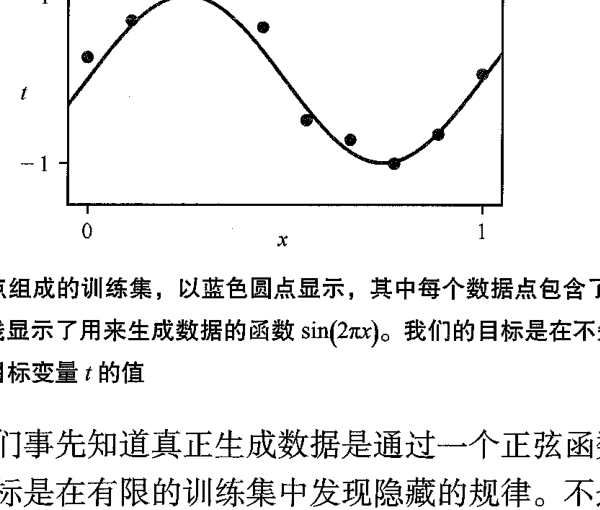
\includegraphics[width=0.6\textwidth]{ch01-fig1-5-sin-training.png}
  \caption{一个由$N=10$个数据点组成的训练集，以蓝色圆点显示，其中每个数据点包含了输入变量$x$及其对应的目标变量$t$的观测值。绿色曲线显示了用来生成数据的函数$\sin(2\pi x)$。我们的目标是在不知道绿色曲线的情况下，预测新的输入变量$x$所对应的目标变量$t$的值。}
  \label{figure:ch01-正弦拟合训练集}
\end{figure}

\subsection{线性模型}\label{subsection:ch01-线性模型}

现在让我们先从一种相对非正式的方式出发，考虑一种基于曲线拟合的简单方法。我们将使用多项式函数来拟合数据，其形式如下：

\begin{align}
  y(x,\mathbf{w}) = w_0 + w_1 x + w_2 x^2 + \cdots + w_M x^M = \sum_{j=0}^{M} w_j x^j
  \label{align:ch01-多项式模型}
\end{align}

其中$M$是多项式的阶数（order），$x^j$表示$x$的$j$次幂。多项式系数$w_0, \cdots, w_M$统称为向量$\mathbf{w}$。注意，尽管多项式函数$y(x,\mathbf{w})$是$x$的非线性函数，但它也是系数$\mathbf{w}$的线性函数。在\cref{align:ch01-多项式模型}中，像这个多项式一样，关于未知参数呈线性的函数具有重要的特性，同时也存在明显的局限性，它们被称为线性模型（linear model）（参见\cref{chapter:ch04-回归}）。

\subsection{误差函数}\label{subsection:ch01-误差函数}

多项式系数的值将通过拟合训练数据来确定，这可以通过最小化误差函数（error function）来实现，该误差函数度量了对于任意给定的$\mathbf{w}$，函数$y(x,\mathbf{w})$与训练集中数据点之间的拟合误差。有一个使用广泛的简单误差函数，即每个数据点$x_n$的预测值$y(x_n,\mathbf{w})$与相应目标值$t_n$之间的差的平方和的二分之一：

\begin{align}
  E(\mathbf{w}) = \frac{1}{2} \sum_{n=1}^{N} \left\{ y(x_n, \mathbf{w}) - t_n \right\}^2
  \label{align:ch01-平方和误差}
\end{align}

其中引入系数$1/2$是为了后续计算方便。稍后我们将从概率论出发推导此误差函数（参见\cref{subsection:ch03-高斯分布}）。注意，这个误差函数是非负的，当且仅当函数$y(x_n,\mathbf{w})$正好通过每个训练数据点时，其值等于零。平方和误差函数的几何解释如\cref{figure:ch01-误差函数几何}所示。

我们可以通过选择能够使$E(\mathbf{w})$尽可能小的$\mathbf{w}$值来解决曲线拟合问题。因为平方和误差函数是系数$\mathbf{w}$的二次函数，其对系数的导数是系数$\mathbf{w}$的线性函数，所以该误差函数的最小化有一个唯一解，记为$\mathbf{w}^*$，可以通过解析形式求得封闭解（也叫解析解）（参见\cref{section:ch04-线性回归}）。最终的多项式由函数$y(x,\mathbf{w}^*)$给出。

\subsection{模型复杂度}\label{subsection:ch01-模型复杂度}

我们还面临选择多项式的阶数$M$的问题，这将引出模型比较（model comparison）或模型选择（model selection）这一重要概念。\begin{figure}[htbp]
  \centering
  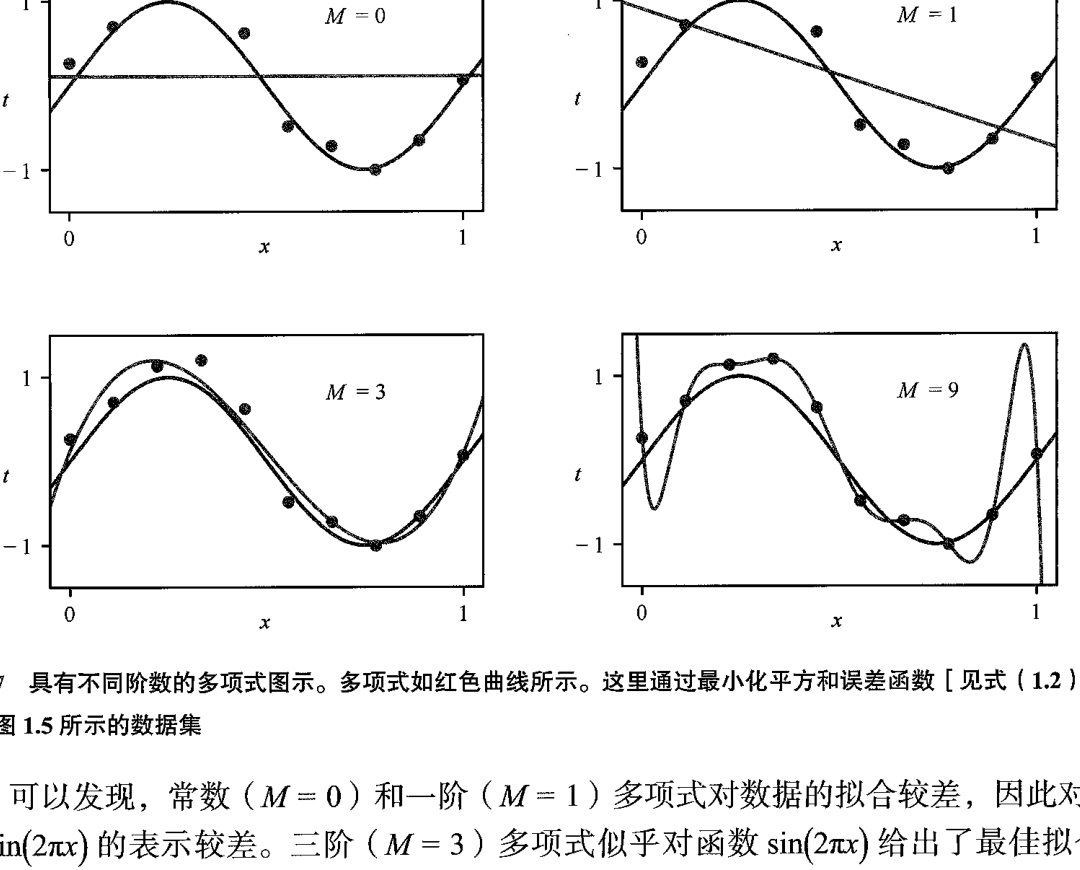
\includegraphics[width=0.8\textwidth]{ch01-fig1-7-poly-fits.png}
  \caption{具有不同阶数的多项式图示。多项式如红色曲线所示。这里通过最小化平方和误差函数（见\cref{align:ch01-平方和误差}）来拟合\cref{figure:ch01-正弦拟合训练集}所示的数据集。}
  \label{figure:ch01-不同阶数拟合}
\end{figure}

在\cref{figure:ch01-不同阶数拟合}中，我们展示了4个拟合实例，它们分别使用阶数$M=0, 1, 3, 9$的多项式来拟合\cref{figure:ch01-正弦拟合训练集}所示的数据集。

可以发现，常数（$M=0$）和一阶（$M=1$）多项式对数据的拟合较差，因此对函数$\sin(2\pi x)$的表示较差。三阶（$M=3$）多项式似乎对函数$\sin(2\pi x)$给出了最佳拟合。高阶（$M=9$）多项式得到了一个对训练数据完美的拟合。事实上，这个多项式曲线精确地穿过了每一个数据点，使得误差$E(\mathbf{w}^*)=0$。然而，拟合出的曲线却出现了剧烈的波动，完全不能反映出函数$\sin(2\pi x)$的真实形态。这种现象称为过拟合（over-fitting）。

我们的目标是让模型获得良好的泛化能力，使其能够对新的数据做出准确的预测。为了定量地探究泛化性能与模型复杂度$M$之间的依赖关系，我们可以引入一个独立的测试集。该测试集包含100个数据点，其生成方式与训练集相同。针对每一个$M$值，我们不仅可以计算出模型在训练集上的残差$E(\mathbf{w}^*)$（\cref{align:ch01-平方和误差}），还可以计算出其在测试集上的残差$E(\mathbf{w}^*)$。与评估误差函数$E(\mathbf{w})$相比，有时使用均方根（Root Mean Square, RMS）误差更为方便，均方根误差定义如下：

\begin{align}
  E_{\mathrm{RMS}} = \sqrt{\frac{1}{N} \sum_{n=1}^{N} \left\{ y(x_n, \mathbf{w}^*) - t_n \right\}^2}
  \label{align:ch01-RMS误差}
\end{align}

公式中的$1/N$是为了让不同大小的数据集能够在相同的基准下进行比较，而求平方根则是为了确保$E_{\mathrm{RMS}}$是在与目标变量$t$相同的尺度上（以相同的单位）进行测量的。

\cref{figure:ch01-误差曲线}展示了不同$M$值的训练集和测试集的RMS误差图。测试集上的RMS误差反映了我们根据新观测数据$x$预测其对应$t$值的能力。从图中可以看出，当$M$值较小时测试集误差较大，这是因为此时的多项式模型灵活性不足，无法捕捉函数$\sin(2\pi x)$中的振荡。当$M$取值在$[3, 8]$时，测试集误差较小，同时这些模型也能合理地表示出数据的生成函数$\sin(2\pi x)$，如\cref{figure:ch01-不同阶数拟合}中$M=3$时所示。

此外，我们或许会认为，预测新数据的最佳模型就应该是生成这些数据的真实函数$\sin(2\pi x)$本身（我们后续将验证这一点）。同时，我们知道$\sin(2\pi x)$的幂级数展开式中包含了所有阶数的项，所以我们会很自然地推断，随着模型复杂度$M$的增加，预测效果应该会持续提升。

通过观察\cref{table:ch01-多项式系数}中不同阶数多项式拟合得到的系数$\mathbf{w}^*$，我们可以更深入地了解这个问题。我们注意到，随着$M$的增加，系数的幅度越来越大。特别是当$M=9$时，为了让对应的多项式曲线能精准地穿过每一个数据点，这些系数被精细地调整到了很大的正值或负值。但在数据点之间，尤其是在数据范围的两端附近，曲线却出现了大幅度的摆动，正如我们在\cref{figure:ch01-不同阶数拟合}中看到的那样。直观地看，当多项式模型具有较大的$M$值时，它变得更加灵活，从而更容易受到目标值上随机噪声的影响，并过度拟合了这些噪声。

为进一步探究该现象，我们观察随着数据集大小的变化，模型学习效果的相应变化，如\cref{figure:ch01-数据集大小影响}所示。可以看出，当模型复杂度固定时，数据集越大，过拟合现象就越不明显。换言之，数据量越大，我们就能用越复杂（即更灵活）的模型去拟合数据。

\subsection{正则化}\label{subsection:ch01-正则化}

根据可用训练集的大小来限制模型中参数的数量，其结果有些不尽如人意。而根据待解决问题的复杂性来选择模型的复杂性似乎更合理。作为限制参数数量的替代方案，正则化（regularization）技术经常被用于控制过拟合现象，它通过向误差函数添加一个惩罚项来抑制系数取值过大。最简单的惩罚项采用所有系数的平方和的形式，误差函数变为

\begin{align}
  \tilde{E}(\mathbf{w}) = \frac{1}{2} \sum_{n=1}^{N} \left\{ y(x_n, \mathbf{w}) - t_n \right\}^2 + \frac{\lambda}{2} \sum_{j=0}^{M} w_j^2
  \label{align:ch01-正则化误差}
\end{align}

其中$\|\mathbf{w}\|^2 = \mathbf{w}^{\mathsf{T}} \mathbf{w} = w_0^2 + w_1^2 + \cdots + w_M^2$，并且系数$\lambda$控制着正则化项与平方和误差项之间的相对重要性。注意，正则化项中通常不包含系数$w_0$，因为如果包含$w_0$，就会导致最终结果受到目标变量所选原点的影响（Hastie, Tibshirani, and Friedman, 2009）。当然也可以包含$w_0$，但需要单独为其配置一个正则化系数（参见\cref{subsection:ch09-参数范数惩罚}）。同样，我们可以求得\cref{align:ch01-正则化误差}中误差函数的精确闭式解（见习题4.2）。在统计学文献中，这类方法被称为收缩方法（shrinkage），因为它们会使系数的值缩小。在神经网络领域，这种方法称为权重衰减（weight decay），因为神经网络中的参数通常称为权重，而这种正则化手段会促使这些权重向零衰减。

\cref{figure:ch01-正则化拟合}展示了采用正则化误差函数（\cref{align:ch01-正则化误差}）对9阶（$M=9$）多项式进行拟合的结果，所用数据集与之前相同。观察发现，当取$\ln \lambda = -18$时，过拟合现象被有效抑制，此时的拟合曲线与目标函数$\sin(2\pi x)$相当接近。反之，若$\lambda$取值过大，则会导致欠拟合，如\cref{figure:ch01-正则化拟合}中$\ln \lambda = 0$的情形。\cref{table:ch01-正则化系数}给出了不同$\lambda$值下拟合得到的多项式系数，这些数值表明，正则化确实发挥了预期作用，有效减小了系数的幅度。

通过绘制训练集和测试集的RMS误差（\cref{align:ch01-RMS误差}）与$\ln \lambda$的关系，可以看出正则化项对泛化误差的影响，如\cref{figure:ch01-正则化参数影响}所示。可以看到，$\lambda$现在控制了模型的有效复杂性，从而决定了过拟合的程度。

在本例中，$\lambda$作为一个超参数（hyperparameter），它的值在基于误差函数最小化来确定模型参数$\mathbf{w}$的过程中始终保持不变。需要注意的是，我们不能通过同时对$\mathbf{w}$和$\lambda$最小化误差函数的方式来简单地确定$\lambda$的取值，因为这样会导致$\lambda$趋近于0，从而产生过拟合。

\subsection{模型选择}\label{subsection:ch01-模型选择}

交叉验证的主要缺点在于所需的训练次数增加了$S$倍，这对于训练过程本身计算成本较高的模型来说是一个大问题。交叉验证等使用独立数据评估性能的技术还存在另一个问题，即对于单个模型可能存在多个复杂度超参数（例如，可能有多个正则化超参数）。在最坏的情况下，探索这些超参数设置的最佳组合可能需要指数级数量的训练次数。现代机器学习的前沿领域需要非常大的模型和大规模训练数据集。因此，超参数设置的探索空间有限，很大程度上依赖于从小模型获得的经验和启发式方法。

这个将多项式模型拟合到基于正弦函数生成的合成数据集的简单示例，阐释了机器学习领域的一些核心概念，在后续章节我们将进一步用这个示例进行讨论。然而，现实中的机器学习应用往往要复杂得多：首先，用于模型训练的数据集规模可能会非常庞大，数据量通常会高出几个数量级；其次，模型的输入变量的数量通常也会显著增加，例如，在图像分析领域，输入变量的规模可达百万量级，并且还可能伴随着多个输出变量。在这些应用中，将输出映射到输入的可学习函数通常由一类被称为神经网络的模型来表征，这些模型往往具有海量的参数，其数量甚至可以达到千亿的规模。此时，误差函数将表现为这些模型参数的复杂非线性函数，无法再通过闭式解的方式进行最小化，而必须借助迭代优化的方法，利用误差函数关于模型参数的导数信息来逐步逼近最优解。这对计算机硬件提出了更高的要求，并且在实际应用中不可避免地会引入相当高的计算成本。

\end{document}